\chapter{Implementation}%
\label{chp:implementation}

\section{Tooling, Environment, and Data Acquisition}%
\label{sec:impl_tooling}

All stages within the pipeline are developed entirely in Python~3. OpenCV is used throughout for image processing including reading images, colour space conversion, and homography computation. Player detection and segmentation are performed using the Ultralytics library with the YOLO11x-seg pretrained weights. Player kit colour is identified by running K-Means clustering using scikit-learn. Clip extraction relies on FFmpeg invoked as a subprocess, and the SoccerNet Python package is used to download match video files and to parse event annotations. The three annotation interfaces are served by Python's built-in \texttt{http.server} module and share a common architecture: a single-page HTML application is served locally, the browser communicates with the Python backend via fetch requests to JSON endpoints, and state is written to disk only on operator confirmation. Completed frames are loaded on startup and skipped, so any session can be interrupted and resumed without loss of work. All intermediate outputs --- keyframe indices, player detections, landmark correspondences, homography matrices, and offside verdicts --- are stored to disk as JSON files, so that every stage can be rerun independently.

Match footage is obtained through the SoccerNet API. For each downloaded match, the event annotation file is parsed to identify all offside events, each carrying a timestamp in milliseconds. For each offside event a short clip is then extracted using FFmpeg: 10 seconds before the timestamp and 25 seconds after, summing up to a 35-second window which would possibly contain both the live moment and any broadcast replay of the offside event. For any already extracted clip, it is skipped and not extracted again to avoid any redundancy.

\section{Keyframe Annotation Interface}%
\label{sec:impl_keyframe}

From each extracted clip the operator must identify the single frame at which the ball leaves the passer's foot. A browser-based annotation interface (\texttt{annotate\_keyframes.py}, port~5000) was developed for this purpose. It loads all frames from a clip into memory using OpenCV, serves individual frames as base64-encoded JPEGs, and provides single-frame, ten-frame, and twenty-five-frame navigation together with a timeline scrubber. The operator marks the chosen frame with a button press or keyboard shortcut, or skips the clip entirely if the relevant players are not visible. The annotation state is persisted after every user interaction, allowing the operator to resume an interrupted session at any point. A separate script then exports the marked JPEG keyframe from each clip.

\section{Player Detection and Team Identification}%
\label{sec:impl_team_id}

YOLO11x-seg is run on each keyframe to produce bounding boxes and per-pixel segmentation masks for all detected persons. The segmentation variant is used because the mask allows kit colour extraction to sample only pixels belonging to the player's body, rather than the background included in a plain bounding box crop.

Detection is performed in two passes to balance precision and recall across the depth of the pitch. A primary pass at confidence 0.3 with an NMS IoU threshold of 0.7 collects all person detections above an adaptive minimum height. The 0.3 confidence floor removes low-quality detections while retaining players at medium distances; the 0.7 NMS IoU threshold (the Ultralytics default) suppresses duplicate boxes of the same player without merging adjacent players standing close together. The minimum height threshold is set adaptively based on the median detected player height in the primary pass: if the median is below 45 pixels (indicating a wide-angle view with many distant players), the minimum is set to 20 pixels to retain small far-end detections; otherwise it is set to 40 pixels to filter non-player noise. These height values were calibrated empirically against the annotated keyframe set to balance retention of legitimate far-end players against rejection of noise detections. A secondary pass at confidence 0.05 is then run; only detections whose bounding box centre falls in the upper \texttt{top\_zone} fraction of the frame are accepted, targeting the far end of the pitch where perspective compression makes distant players appear smaller than the primary pass minimum height. Duplicate detections between passes are suppressed by an IoU overlap check with a threshold of 0.4 --- looser than the NMS threshold to account for the fact that far-end boxes are small and overlap estimates are noisier. Detections near the touchline, in image corners, or at the very bottom of the frame are subsequently classified as non-pitch personnel and excluded from the team identification step. Evaluated across the full 164 annotated keyframes in the dataset, the secondary pass contributed 499 additional detections that the primary pass missed, affecting 139 of 164 frames (84.8\%). On affected frames the secondary pass recovered an average of 3.6 additional players per frame, with a maximum of 15 in a single frame. These recovered players are disproportionately defenders near the far end of the pitch, whose position along the offside line makes their inclusion critical to a correct verdict.

For each remaining detection, a torso region of interest is defined by restricting the crop vertically to between 20\% and 60\% of the bounding box height, skipping the head and legs. A horizontal trim of 18\% is applied to each side of the crop to reduce contamination from arm skin and sleeve edges. Pixels in this region whose colour in \gls{hsv} space falls within the grass green range are excluded; the grass colour is estimated from the image by masking the field and computing the mean BGR value. \gls{hsv} is used at this stage because grass occupies a compact, well-defined hue band that can be isolated with a simple range check, and the binary grass/not-grass decision does not require perceptually uniform distances. The remaining pixels are converted to CIE Lab for feature extraction: unlike \gls{hsv}, CIE Lab is perceptually uniform, meaning Euclidean distances correspond to perceived colour differences, which is a necessary property for K-Means clustering to group players by visually similar kit colours rather than by arbitrary numerical proximity. The pixels are summarised by the six-dimensional feature vector shown in Listing~\ref{lst:feature}.

\begin{lstlisting}[language=Python, caption={Construction of the six-dimensional kit colour feature vector.}, label={lst:feature}]
median_L = np.median(L)
median_a = np.median(a)
median_b = np.median(b)
dark_ratio  = np.mean(L < 80)
bright_ratio = np.mean(L > 150)
sat_proxy = np.median(np.sqrt((a - 128)**2 + (b - 128)**2))
size_factor = min(1.0, (height * width) / 8000)
return np.array([median_L, median_a, median_b,
                 dark_ratio * 100 * size_factor,
                 bright_ratio * 100, sat_proxy])
\end{lstlisting}

Three aspects of the feature vector construction require explanation. First, the saturation proxy is computed as $\text{median}\!\left(\sqrt{(a^* - 128)^2 + (b^* - 128)^2}\right)$ rather than simply $\sqrt{(a^*)^2 + (b^*)^2}$: OpenCV encodes CIE Lab so that the achromatic (neutral grey) point lies at $(a^*, b^*) = (128, 128)$, not at the origin, so the subtraction re-centres the distance measurement at the true neutral point. Without this correction the saturation proxy would measure distance from a corner of the colour space rather than from achromatic, producing incorrect saturation estimates for dark kits. Second, the \texttt{size\_factor} scales the dark-ratio dimension by $\min(1,\, h \times w\, /\, 8000)$, where $8000\,\text{px}^2$ corresponds approximately to the bounding box area of a player at mid-distance in a broadcast frame ($\approx 90 \times 90$\,px). Small distant players have a proportionally larger fraction of background pixels in their crop, producing noisier colour estimates; down-weighting the dark-ratio dimension for small boxes reduces their influence on the cluster centroids. Third, grass pixels are excluded using an HSV mask with hue range $[35^\circ, 85^\circ]$, saturation above 40 and value above 40 (both on OpenCV's 0--255 scale, where saturation measures colour intensity and value measures brightness, so these thresholds exclude near-grey and near-black pixels respectively), which covers the full range of natural and broadcast-lit grass colours while avoiding false positives on yellow or white kit elements.

Prior to clustering with K-Means, players likely to belong to referees, goalkeepers, or other non-outfield categories are pre-flagged and excluded from clustering. A player is pre-flagged under two conditions: (i)~their L* is below 50 (nearly black), indicating a referee kit, provided they are not chromatically consistent with at least two other players (which would suggest a dark team kit rather than an official); or (ii)~their L* is below 100 and their chromaticity is below a saturation of 13, capturing the low-saturation dark grey typical of referees. A separate check flags any player whose $(a^*, b^*)$ chromaticity has fewer than two similar neighbours within a radius of 15 units in $a^*b^*$ space as colour-isolated, removing outlier kits not shared by at least two others. A mini-team rescue pass prevents a small team visible in only three players from being entirely flagged: if three or more isolated players are mutually within a chroma radius of 22 they are restored to the clustering pool, as they form a coherent group rather than scattered officials.

All numeric thresholds (torso crop boundaries, HSV grass mask, OTH pre-flag bounds, neighbourhood radii) were determined empirically via iterative visual inspection. Per-parameter ablation is infeasible without per-player ground-truth labels, which SoccerNet does not provide; instead the thresholds were tuned during initial development on a small subset of frames and then held fixed for the full 164-frame evaluation. The 2.0\% end-to-end team misidentification rate measured across that broader, untouched set indicates that the chosen values generalise rather than overfit to the development subset.

With the remaining players, K-Means with $k=2$ is applied to the standardised feature vectors. The choice of $k=2$ reflects the domain constraint that exactly two outfield teams are present in any match. Setting $k=3$ to absorb referees and goalkeepers directly was considered but rejected: because kit colour variation within a team (due to lighting, shadow, and distance) can exceed the colour difference between a referee's kit and one of the teams, a third cluster frequently captures within-team variation rather than officials, producing a degenerate split. Pre-flagging non-outfield personnel before clustering and enforcing $k=2$ on the remainder is more robust. Before clustering, features are normalised with \texttt{StandardScaler} and the $a^*$ and $b^*$ chroma channels are then multiplied by 1.8 to re-emphasise hue over brightness. This is necessary because K-Means implicitly assumes clusters of equal isotropic variance in feature space, so any dimension with greater raw spread tends to dominate the cluster boundary regardless of how discriminative it is; in football broadcasts the L* (brightness) channel varies strongly with shadow and camera angle while shirt hue is consistent, so unweighted clustering reliably splits on brightness rather than team colour. The 1.8 weight was selected empirically and balances chroma dominance without overwhelming the remaining dimensions. K-Means is run five times with different random seeds and the result with the most balanced cluster sizes is retained; the balance score is $\min(c_0, c_1)\,/\,\max(c_0, c_1)$, where $c_0$ and $c_1$ are the cluster sizes, giving 1.0 for a perfect 50/50 split. This multi-start strategy guards against the known sensitivity of K-Means to initialisation, particularly when the two team colours are close together in Lab space. The resulting team assignments for a representative keyframe are shown in Figure~\ref{fig:team_id}.

\begin{figure}[h]
  \centering
  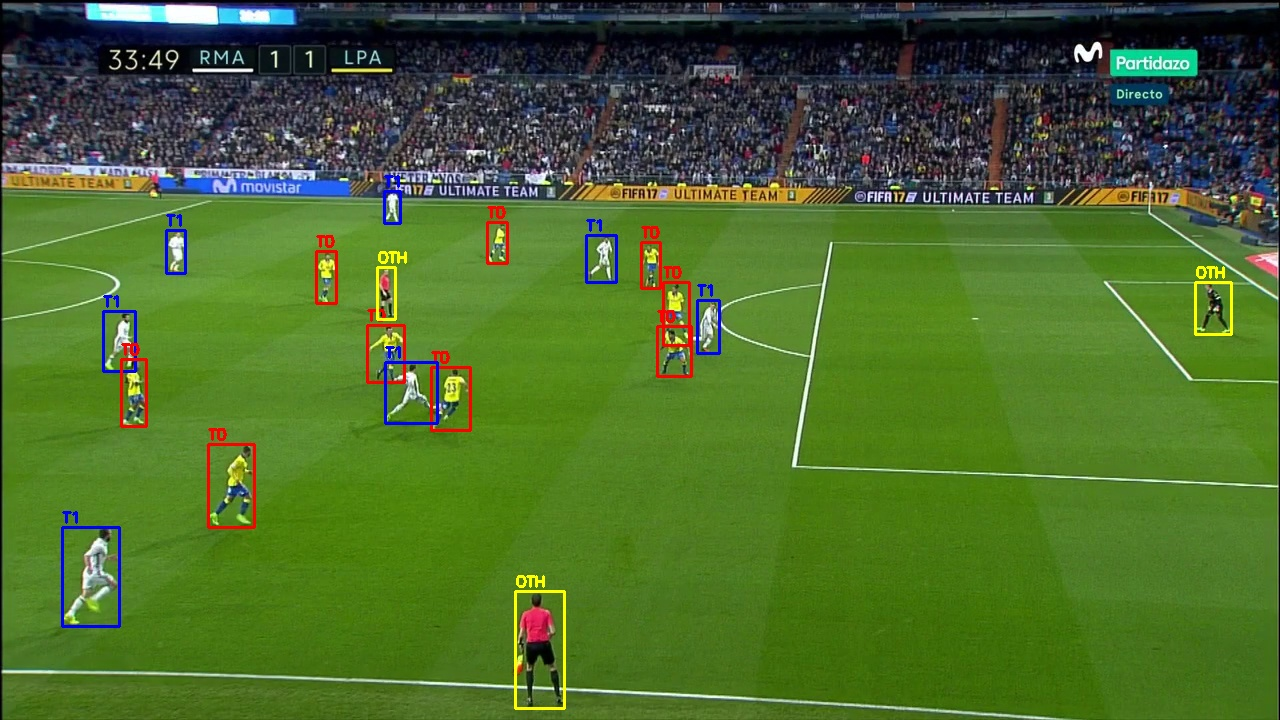
\includegraphics[width=0.9\linewidth]{content/chapters/4_implementation/figures/team_identification_figure.jpg}
  \caption{YOLO11x-seg detections with K-Means clustering team assignment. Blue boxes indicate Team~1, red boxes Team~0, and yellow indicates an OTH (referee/goalkeeper/non-outfield detection). Labels show the detection index and cluster assignment.}
  \label{fig:team_id}
\end{figure}

\section{Homography Estimation}%
\label{sec:impl_homography}

Pitch landmark correspondences are collected through a browser-based interface (\texttt{pick\_points.py}, port~5001). The interface serves each keyframe image and captures click coordinates from the browser, displaying a live table of entered correspondences. Each recorded point is further refined to subpixel precision using OpenCV's \texttt{cornerSubPix} function, which iteratively repositions the click to the nearest intensity-gradient corner within a $7\times7$ pixel search window. The iterative refinement runs for at most 30 iterations and terminates early if the point moves less than 0.01 pixels between steps, balancing precision against computational cost. Refinement is skipped if the click falls within 2 pixels of the image edge, where the search window would extend outside the image boundary. The operator then selects the corresponding landmark on an interactive pitch diagram to provide the real-world coordinate, and must submit at least four correspondences before the frame is accepted --- four being the theoretical minimum: $\mathbf{H}$ has eight degrees of freedom (nine matrix entries, minus one for the scale ambiguity), and each point correspondence contributes exactly two independent linear constraints, so four correspondences are needed to make the system fully determined.

The homography is estimated using a two-stage process, illustrated in Listing~\ref{lst:homography}. The first pass applies RANSAC with a reprojection threshold of 2.0\,m to identify a consistent inlier set. RANSAC was preferred over the alternative robust estimator LMedS (\texttt{cv2.LMEDS}), which minimises the median squared residual and requires no threshold, because the explicit threshold of RANSAC can be reasoned about directly in terms of expected click precision, making the choice transparent and adjustable; LMedS offers no equivalent handle. This threshold was chosen to match the precision achievable with manual landmark clicks: at the far touchline, where perspective compression is greatest, one pixel corresponds to approximately 0.06\,m, making the practical click precision of $\pm$10--15\,pixels equivalent to $\pm$0.6--0.9\,m of world-space error. A threshold of 2.0\,m therefore accepts all reasonably-placed clicks while still rejecting gross outliers such as misidentified landmarks. The second pass refits $\mathbf{H}$ from only the RANSAC inlier set via ordinary least squares (\texttt{method=0}), which is the maximum-likelihood estimate under Gaussian noise and produces a tighter solution than the RANSAC homography alone.

\begin{lstlisting}[language=Python, caption={Two-pass homography estimation: RANSAC followed by least-squares refit on inliers.}, label={lst:homography}]
H_ransac, mask = cv2.findHomography(
    image_pts, real_pts, cv2.RANSAC,
    ransacReprojThreshold=2.0)

inliers_mask = mask.ravel().astype(bool)
if inliers_mask.sum() >= 4:
    H, _ = cv2.findHomography(
        image_pts[inliers_mask],
        real_pts[inliers_mask],
        method=0)   # ordinary least squares
\end{lstlisting}

A homography is defined only up to scale, meaning $\mathbf{H}$ and $-\mathbf{H}$ represent the same projective transformation. However, only one sign produces valid (positive projective denominator) projections for points on the physical pitch plane; the opposite sign maps those points to the geometrically mirrored half-space, producing sign-flipped world coordinates. After estimation, the sign of $\mathbf{H}$ is normalised by checking the projective denominator at the centroid of the picked image points: if the denominator is negative, $\mathbf{H}$ is negated. This step is necessary to guarantee that world-space $x$-coordinates produced by the system carry the correct sign for the offside comparison.

A final quality gate is applied before a frame is passed to the offside checker: a $12 \times 8$ grid of sample points is projected through $\mathbf{H}$ across the player zone of the image, and the fraction with a non-positive projective denominator is recorded. Frames where more than 15\% of the player zone produces invalid projections are automatically excluded, as the homography is not well-conditioned enough to support reliable player position estimates across the full pitch. The 15\% threshold was determined empirically as the value that correctly excluded near-singular homographies while retaining all frames with geometrically valid calibrations.

The quality of each estimated homography is reported as the symmetric pixel reprojection error: the known world coordinates of each correspondence are transformed back into the image via $\mathbf{H}^{-1}$ and the Euclidean distance to the original click position is measured. A validation overlay is also rendered for each keyframe by projecting the full FIFA pitch line model through $\mathbf{H}^{-1}$; the resulting lines should align with the visible pitch markings, making any gross calibration error immediately apparent, as illustrated in Figure~\ref{fig:homography_validation}.

\begin{figure}[h]
  \centering
  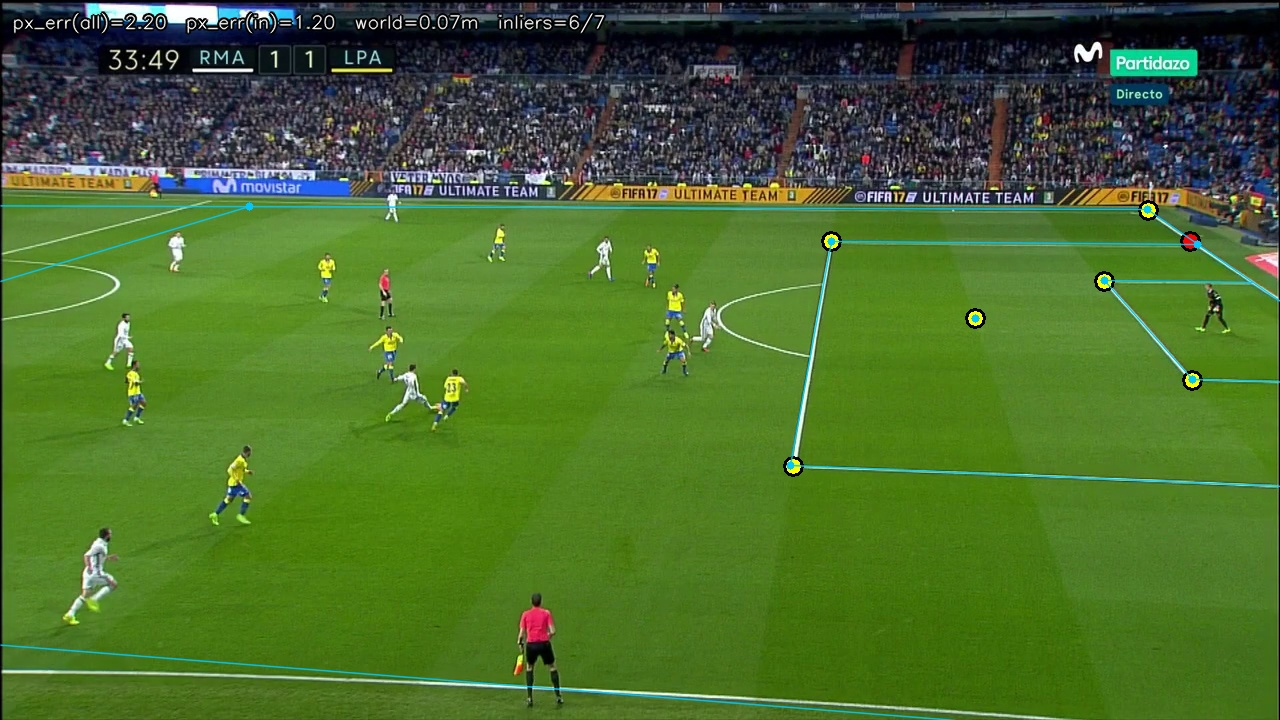
\includegraphics[width=0.9\linewidth]{content/chapters/4_implementation/figures/homography_validation_figure.jpg}
  \caption{Homography validation overlay: the FIFA pitch line model is projected back into the image via $\mathbf{H}^{-1}$ and rendered in cyan. Close alignment with the visible pitch markings confirms a consistent calibration.}
  \label{fig:homography_validation}
\end{figure}

\section{Offside Decision}%
\label{sec:impl_offside}

The offside checker interface (port~5002) accepts the operator-specified attacking team, direction of attack, and attacker index. All defending players' foot positions are projected through $\mathbf{H}$ into world coordinates; before ranking, any defender whose projected position falls outside the FIFA pitch boundary ($|X| \leq 52.5$\,m, $|Y| \leq 34$\,m with a small margin) is excluded, as this indicates a touchline steward or pitch-side official that YOLO has detected as a person rather than an outfield player. The most advanced remaining defender along the direction of attack is taken as the second-to-last defender.

The foot position used for both attacker and defender is the bottom corner of the bounding box on the side facing the direction of attack: the right-edge foot $(x_2, y_2)$ when attacking right, and the left-edge foot $(x_1, y_2)$ when attacking left. This measures the leading edge of each player's ground contact region, consistent with the body-part interpretation of Law~11. Both points are projected through $\mathbf{H}$ to give world coordinates $(X_{\text{att}},\, Y_{\text{att}})$ and $(X_{\text{def}},\, Y_{\text{def}})$. The signed margin $m = d\cdot(X_{\text{att}} - X_{\text{def}})$ is then computed, where $d \in \{+1, -1\}$ encodes the direction of attack as detected from the homography axis orientation. A positive $m$ indicates the attacker is ahead of the defender (offside); a negative $m$ gives onside. The magnitude $|m|$ is reported in metres. The offside line is rendered by inverting $\mathbf{H}$ at the defender's world $x$-coordinate to obtain two image-space points, which are connected with a line overlay across the full height of the frame.

\section{Challenges Encountered}%
\label{sec:impl_challenges}

Several implementation problems arose that required significant revision of the initial design.

\textbf{Insufficient player detection.} The initial implementation used YOLO11m, which frequently missed detections in the far half of the pitch where distant players appear small. Replacing it with YOLO11x-seg improved recall for small and partially occluded players: across all evaluation keyframes, YOLO11x-seg produced on average 0.8 additional detections per frame. The segmentation masks further allowed colour extraction to sample only pixels inside the player's outline rather than the rectangular bounding box crop.

\textbf{Kit colour contamination.} Early team identification used the median Lab colour of a simple bounding box crop, which included arm skin and shorts contamination. Three refinements addressed this: a vertical restriction to the upper-middle torso region, an 18\% horizontal trim, and grass-colour exclusion via HSV masking. The combined effect is reflected in the evaluation: team misidentification accounted for only 3 of the 150 clean events (2.0\%), attributable to spectrally similar kits rather than contamination.

\textbf{OTH classifier over-flagging outfield players.} The initial approach used simple luminance thresholds to identify referees and goalkeepers, which frequently misclassified outfield players in dark or unusual kits as officials. Outlier detection was rebuilt around the modified Z-score $\tau = \tilde{d} + 3.5 \cdot 1.4826 \cdot \mathrm{MAD}$~\cite{iglewicz1993outliers}, where $\tilde{d}$ is the median centroid distance and $1.4826$ is the standard consistency factor relating the \gls{mad} (a robust, outlier-resistant measure of spread) to the standard deviation of a Gaussian. A player is flagged OTH only when their distance exceeds $\tau$ \emph{and} they are not clearly assigned to one team. A bimodal chroma refit handles frames where K-Means splits on brightness rather than hue.

\textbf{Insufficient landmark coverage.} The initial landmark set (halfway line, penalty box corners, centre circle) proved insufficient for frames where the camera is near one end of the pitch. The set was extended to include 6-yard box corners, goalpost bases, and corner flags, which are visible in nearly all valid broadcast frames and improved both inlier count and reprojection error.

\textbf{RANSAC threshold calibration.} The initial threshold of 0.5\,m proved too strict: at the far touchline, one pixel corresponds to approximately 0.06\,m, making 0.5\,m equivalent to only $\pm$8 pixels of tolerated click error. Since manual clicks achieve $\pm$10--15 pixels, the threshold routinely rejected correctly-placed correspondences, leaving the homography under-constrained where the offside line typically lies. Relaxing to 2.0\,m accommodates realistic click imprecision while still rejecting gross misidentifications --- a wrongly-clicked landmark is typically displaced by 50--100 pixels or more. Across 162 calibrated frames this produced a mean inlier ratio of 94.5\%, confirming that most correspondences are accepted.

\textbf{Image-space defender ranking and reprojection error metric.} Ranking by image-space x-coordinate fails on oblique cameras; projecting foot positions through $\mathbf{H}$ resolves this. World-space residuals in metres were replaced by the symmetric pixel reprojection error of Section~\ref{sec:impl_homography}, which is consistent at all depths.
